\chapter{Compression de Signaux}
\label{comp-code-chap}

La compression de signaux s'apparente \`a la deshydratation d'un
litre de jus d'orange en quelques grammes de poudre concentr\'ee.
Le go\^ut de la boisson orange restitu\'ee est similaire au jus d'orange
mais a souvent perdu de sa subtilit\'e.
En traitement du signal, nous sommes plus interess\'es
par des sons ou des images, mais l'on rencontre le m\^eme
conflit entre qualit\'e et compression.
Minimiser la d\'egradation pour un taux de compression donn\'e est
le but des algorithmes de codage.
Les applications principales concernent le stockage des donn\'ees
et la transmission \`a travers des canaux \`a d\'ebit limit\'e.

Nous \'etudions les algorithmes de codage
qui d\'ecomposent le
signal sur une base orthogonale et approximent efficacement les
coefficients de d\'ecomposition.
Ce type de codage est actuellement le plus performant pour
restituer des signaux audios ou des images de bonne qualit\'e.

\section{Codage compact}

La performance ultime d'un algorithme de codage est mesur\'ee par
un ``score d'opinion moyen''.
Pour un taux de compression donn\'e,
la qualit\'e des signaux cod\'es est \'evalu\'ee par plusieurs personnes
et calibr\'es selon une proc\'edure pr\'ecise.
De telles \'evaluations sont longues \`a faire et les r\'esultats
difficiles
\`a interpr\'eter math\'ematiquement. La qualit\'e d'un algorithme de codage
est donc le plus souvent optimis\'ee avec une distance qui
a une forme analytique simple et qui tient compte partiellement de
notre sensibilit\'e visuelle ou auditive.
La distance euclidienne, bien que relativement
grossi\`ere d'un point de vue perceptuel,
a l'avantage d'\^etre facile \`a manipuler analytiquement.


\subsection{Etat de l'art}
\label{stateofart}
\noindent
{\bf Parole}
Le codage de la parole est particuli\`erement important pour
la t\'el\'ephonie o\`u il peut \^etre de qualit\'e m\'ediocre tout en
maintenant une bonne intelligibilit\'e.
Un signal de parole par t\'el\'ephone est limit\'e \`a la bande de
fr\'equence 200-3400 Hz et est \'echantillonn\'e \`a 8kHz.
Un ``Pulse Code Modulation (PCM)'' qui quantifie chaque
\'echantillon sur
8 bits produit un code de 64kb/s ($64~10^3$ bits par seconde).
Ceci peut \^etre consid\'erablement r\'eduit en supprimant certaines
composantes redondantes de la parole.

Nous avons vu dans le paragraphe \ref{modelisation-paro} que
la production d'un signal de parole est bien comprise.
Des filtres autor\'egressifs
excit\'es par des trains d'impulsions ou un bruit
blanc Gaussien
permettent de restaurer un signal
intelligible \`a partir de peu de param\`etres.
Ces codes d'analyse-synth\`ese, tel que le standard LPC-10 d\'ecrit
dans le paragraphe \ref{compre-LPC},
produisent un signal de parole intelligible
\`a 2,4kb/s. \\

{\bf Audio}
Les signaux audios peuvent inclure de la parole mais aussi de la
musique et n'importe quel type de son.
Ils sont donc beaucoup plus difficiles \`a mod\'eliser que la parole.
Sur un disque compact, le signal audio est limit\'e \`a un maximum
de 20kHz. Il est \'echantillonn\'e \`a 44.1kHz et chaque \'echantillon est
cod\'e sur 16bits. Le d\'ebit du code PCM r\'esultant est donc de
706kb/s. Le signal audio d'un disque compact ou d'une cassette
digitale doit \^etre cod\'e sans distortion auditive.

Les codeurs par transform\'ee orthogonale qui d\'ecomposent les
signaux sur des bases locales en temps et en fr\'equence sont
parmi les plus performants pour les signaux audios, car ils ne
n\'ecessitent pas la mise en place d'un mod\`ele.
Une qualit\'e de disque compact est obtenue par des codeurs
n\'ecessitant 128kb/s.
Avec 64kb/s les d\'egradations sont \`a peine audibles.
Ces algorithmes sont particuli\`erement importants pour les
CD-ROM en multim\'edia.\\

{\bf Images}
Une image couleur est compos\'ee de trois canaux d'intensit\'e
dans le rouge, le vert et le bleu.
Chacune de ces images a typiquement
500 par 500 pixels, qui sont cod\'es sur 8 bits (256 niveaux de gris).
Un canal t\'el\'ephonique digital ISDN  a un d\'ebit de 64kb/s.
Il faut donc environ 2 minutes pour transmettre une telle image.

Les images tout comme les signaux audios incluent le plus souvent
des structures de type diff\'erent qu'il est difficile de mod\'eliser.
Courament, les algorithmes de compression les plus efficaces sont
bas\'es sur des transform\'ees orthogonales utilisant des bases de
cosinus locaux ou des bases d'ondelettes.
Avec moins de 1 bit/pixel, ces codes reproduisent une image
de qualit\'e visuelle presque parfaite.
A 0.25 bit/pixel, l'image reste de bonne qualit\'e visuelle et
peut \^etre transmise en 4 secondes sur une ligne t\'el\'ephonique
digitale.

\subsection{Codage dans une base orthogonale}
\label{transf-sec}

Un code orthogonal d\'ecompose le signal dans une base
orthogonale bien choisie de fa\c con \`a optimiser la compression
des coefficients de d\'ecomposition.
La classe des signaux cod\'es est represent\'ee
par un vecteur al\'eatoire $Y[n]$ de taille $N$.
On d\'ecompose $Y[n]$ sur une
base orthogonale $\{ g_m [n] \}_\ZnN$
\[
Y[n] = \sum_{m=0}^{N-1} A[m] \,g_m [n] .
\]
Les coefficients de d\'ecomposition
$A[m]$ sont des variables al\'eatoires
\[
A[m] = <Y[n] , g_m [n] > =
\sum_{n=0}^{N-1} Y[n] \, g^*_m [n] .
\]
Si $A[m]$ n'est pas de moyenne nulle,
on code $A[m] - E\{A[m]\}$ et on m\'emorise la valeur moyenne
$E\{A[m]\}$. Nous supposerons par la suite que
$E\{A[m]\}$ = 0.
\\
\\
{\bf Quantification}
Les valeurs r\'eelles
$\{A[m]\}_\ZmN$ doivent \^etre approxim\'ees avec une pr\'ecision finie
pour construire un code de taille finie.
Une quantification scalaire approxime chaque
$A[m]$ individuellement.
Si les coefficients $A[m]$ ont une forte d\'ependance,
le taux de compression peut \^etre am\'elior\'e
avec une quantification vectorielle qui regroupe les coefficients
en blocs.
Cette approche n\'ecessite cependant plus de calculs.
Si la base $\{ g_m\}_\ZmN$ est choisie de fa\c con \`a ce que
les coefficients $A[m]$ soient presque ind\'ependants,
l'am\'elioration d'une quantification vectorielle est
marginale.

Chaque $A[m]$ est une variable al\'eatoire dont la valeur
quantifi\'ee est $\tilde A[m] = Q_m (A[m])$
Le signal quantifi\'e reconstruit est
\[
\tilde Y[n] = \sum_{m=0}^{N-1} \tilde A[m] \, g_m [n] .
\]
Comme la base est orthogonale
\[
\| Y - \tilde Y \|^2 = \sum_{m=0}^{N-1}
|A[m] - \tilde A[m]|^2
\]
et donc la valeur moyenne de l'erreur est
\[
E\{\| Y - \tilde Y \|^2\} = \sum_{m=0}^{N-1}
E\{|A[m] - \tilde A[m]|^2\}.
\]
Si l'on note
\[
D_m = E\{|A[m] - \tilde A[m]|^2\} ,
\]
l'erreur totale devient
\[
D =  \sum_{m=0}^{N-1}  D_m .
\]
Soit $R_m$ le nombre moyen de bits pour coder $\tilde A [m]$.
Pour une quantification \`a haute r\'esolution,
le th\'eor\`eme \ref{quanti-theo} montre que si
$D_m$ est fix\'e alors on minimise
$R_m$ avec une quantification scalaire uniforme. On note $\Delta_m$
la taille des intervales de quantification. On a montr\'e en
(\ref{unifoquantiz}) que
\[
D_m = \frac {\Delta_m^2} {12} .
\]
et (\ref{lower-quantX}) prouve que
\[
R_m = H_d (X) -  \frac 1 2 \log_2 (12 D_m) =
H_d (X) -  \log_2 \Delta_m ~,
\]
o\`u $H_d (X)$ est l'entropie diff\'erentielle de $X$ d\'efinie
par (\ref{entropie-dffD}).
\\
\\
{\bf Allocation de bits}
Si l'on fixe l'erreur totale $D$, il nous faut
optimiser le choix de $\{\Delta_m\}_\ZmN$
afin de minimiser le nombre total de bits
\[
R  = \sum_{m=0}^{N-1} R_m .
\]
Soit $\bar R = \frac R N$ le nombre moyen de bits par
coefficient.
Le th\'eor\`eme suivant montre que le codage est optimis\'e
lorsque tous les $\Delta_m$ sont \'egaux.

\begin{theorem}
\label{bit-alloc-th}
Pour une quantification haute r\'esolution et une erreur
totale $D$, on minimize $\bar R$ avec
\begin{equation}
\label{allDeltamequal}
\Delta_m^2 = \frac {12\, D} N~~~\mbox{pour $0 \leq m < N$},
\end{equation}
auquel cas
\begin{equation}
\label{dist-rat-gen}
D(\bar R) = \frac N {12} \, 2^{2 \overline H_d} \, 2^{-2 \bar R} ~,
\end{equation}
o\`u $\overline H_d$ est l'entropie diff\'erentielle moyenne
\[
\overline H_d = \frac 1 N \sum_{m=0}^{N-1} H_d (A[m]) .
\]
\end{theorem}

{\bf D\'emonstration} Pour une quantification haute r\'esolution
uniforme, (\ref{bit-rate-uniform}) montre que
\[
R_m = H_d (A[m]) -  \frac 1 2 \log_2 (12 \, D_m ).
\]
Donc
\begin{equation}
\label{valueofR}
\bar R = \frac 1 N \sum_{m=0}^{N-1} R_m =
\frac 1 N \sum_{m=0}^{N-1}  H_d (A[m]) -
\frac 1 N \sum_{m=0}^{N-1}  \frac 1 2 \log_2 (12 \, D_m ).
\end{equation}
Minimiser $\bar R$ revient \`a minimiser
$\sum_{m=0}^{N-1}  \log_2 (12 D_m )$.
En appliquant l'in\'egalit\'e de Jensen (\ref{jensen}) \`a
la fonction concave $\phi(x) = \log_2 (x)$ pour $p_k = \frac 1 N$
on obtient
\[
\frac 1 N \sum_{m=0}^{N-1} \log_2 (12 \, D_m ) \leq
\log_2 \left(\frac {12} N \sum_{m=0}^{N-1} D_m \right) =
\log_2 \left(\frac {12 \, D} N \right)  .
\]
Cette in\'egalit\'e est une \'egalit\'e si et seulement si tous
les $D_m$ sont \'egaux.
Donc $\frac {\Delta_m^2} {12} = D_m = \frac D N$, ce qui
prouve (\ref{allDeltamequal}). On d\'eduit aussi de
(\ref{valueofR}) que
\[
\bar R = \frac 1 N \sum_{m=0}^{N-1}  H_d (A[m]) -
\frac 1 2 \log_2 \left(\frac {12\, D} N \right)
\]
ce qui implique (\ref{dist-rat-gen}). $\Box$

Ce th\'eor\`eme montre que le codage est optimis\'e en
introduisant la m\^eme erreur moyenne
$D_m = \frac {\Delta_m^2} {12} = \frac D N$ dans la direction
de chaque vecteur $g_m$ de la base. Le nombre moyen de bits
$R_m$ pour coder $A[m]$ d\'epend alors seulement
de l'entropie diff\'erentielle:
\begin{equation}
\label{RmOptiBiallO}
R_m = H_d (A[m]) -  \frac 1 2 \log_2 \left(\frac {12 D} N \right) .
\end{equation}
On note $\sigma_m^2$ la variance de $A[m]$, et
$\hat A [m] = \frac 1 {\sigma_m} \, A[m]$ la variable al\'eatoire
normalis\'ee de variance $1$. Un changement de variable dans
l'int\'egrale de l'entropie diff\'erentielle montre que
\[
H_d (A[m]) = H_d (\hat A[m]) + \log_2 \sigma_m~.
\]
L'allocation de bit optimal $R_m$ donn\'e par
(\ref{RmOptiBiallO}) peut donc devenir n\'egative si
la variance $\sigma_m$ est trop petite, ce qui n'est clairement
pas une solution admissible.
En pratique $R_m$ doit \^etre un entier positif mais imposer cette
contrainte suppl\'ementaire ne permet pas de faire un
calcul analytique simple. La formule (\ref{RmOptiBiallO}) n'est donc
utilisable que si les valeurs $\{R_m\}_{0 \leq m < N}$
sont positives et on les
approxime alors par les entiers les plus proches.
\\
\\
{\bf Normes quadratiques pond\'er\'ees\ } \index{Norm!weighted}
Nous avons mentionn\'e qu'une erreur quadratique souvent ne
mesure pas bien l'erreur per\c{c}ue pour des images ou des
signaux audios. Lorsque les vecteurs
$g_m$ sont bien localis\'es en temps/espace et en fr\'equence,
on peut am\'eliorer cette norme
en pond\'erant les erreurs par des poids qui d\'ependent
de la fr\'equence, afin de se rapprocher de notre sensibilit\'e
auditive/visuelle, qui varie avec la fr\'equence du signal.
Une norme pond\'er\'ee est d\'efinie par
\begin{equation}
\label{weight-normed}
D =  \sum_{m=0}^{N-1} \frac{D_m} {w_m^2} ,
\end{equation}
o\`u $\{ w_m^2\}_\ZmN$ sont des constantes.

Le th\'eor\`eme \ref{bit-alloc-th} s'applique
\`a une norme pond\'er\'ee en observant que
\[
D =  \sum_{m=0}^{N-1} D^w_m,
\]
o\`u $D^w_m =  \frac {D_m} {w_m^2}$
est l'erreur de quantification de $A^w [m] = \frac {A[m]} {w_m}$.
Le th\'eor\`eme \ref{bit-alloc-th}
prouve que l'allocation de bits optimale
est obtenue en quantifiant uniform\'ement
tous les $A^w [m]$ avec des intervales de m\^eme tailles $\Delta$.
Cela implique que les
coefficients $A[m]$ sont uniform\'ement quantifi\'es
avec des intervales de taille
$\Delta_m =  {\Delta}\, {w_m}$, et donc
$D_m = \frac {w_m^2 D}  {N}$.
Comme on s'y attendait, en augmentant les poids $w_m$ on
augment l'erreur dans la direction de $g_m$.
La quantification uniform
$Q_{\Delta_m}$ \`a intervales
$\Delta_m$ est souvent calcul\'ee avec un quantificateur
$Q$ qui associe a tout nombre r\'eel l'entier le plus proche:
\begin{equation}
\label{variable-unifo-quan}
Q_{\Delta_m}\Bigl(A[m]\Bigr) = \Delta_m\, Q\left (\frac {A[m]} {\Delta_m}\right) =
{\Delta}\, {w_m}\, Q \left(\frac {A[m]} {\Delta\,w_m}\right) .
\end{equation}

\section{Bases de Cosinus Locaux}

{\bf Choix de la base}
Le codage d'une classe de signaux $Y[n]$ dans une base
orthogonale $\{g_m [n]\}_\UmN$ est d'autant meilleur que la base
supprime les corr\'elations entre les coefficients $Y[n]$.
La base $\{g_m [n]\}_\UmN$ est donc choisie de fa\c con \`a obtenir des
coefficients $A[m] = <Y,g_m>$ aussi d\'ecorrel\'es que possible.
De m\^eme il est souvent d\'esirable d'obtenir des coefficients
$A[m]$ qui ont une forte probabilit\'e d'\^etre proches de z\'ero.
De tels coefficients sont en effet annul\'es par la quantification
et efficacement cod\'es par en s\'equences.
Les bases de cosinus d\'ecrites dans ce paragraphe sont bien
adapt\'ees pour le codage des signaux audios et des images.
L'existence d'algorithmes de calcul rapide bas\'es sur la transform\'ee
de Fourier rapide permet d'utiliser ces bases pour du codage
en temps r\'eel.
\\
\\
{\bf Bases de Cosinus}
Le codage de signaux r\'eels
$f[n]$ defini pour $0 \leq n < N$
se fait plut\^ot sur des bases de
cosinus que sur des bases de Fourier discr\`etes
$\{\frac 1 {\sqrt N} e ^{\frac {i2 \pi k n} N } \}_\ZkN$.
En effet nous avons vu dans le paragraphe \ref{transf-four-discr}
que la d\'ecompositon d'un signal de taille $N$ dans une base
de Fourier discr\`ete effectue une p\'eriodisation de $f[n]$ sur
$N$ \'echantillons. Si $f[0] \neq f[N-1]$, ce signal p\'eriodique
a des transitions brutales en $n=0$ et $n=N-1$ ce qui produit des
coefficients de Fourier de large amplitude. La quantification
de ces coefficients de large amplitude cr\'ee des erreurs aux
bords que l'on veut \'eviter.
On montre que la base
de cosinus sp\'ecifi\'ee par le Th\'eor\`eme
\ref{th-discr-cos} poss\`ede essentiellement
les m\^emes propri\'et\'es
qu'une base de Fourier discr\`ete, mais ne
produit
pas des coefficients de large amplitude par effet de bord.
Cette base de cosine est bas\'ee sur une extension $\tilde f [n]$
p\'eriodique de $f[n]$,
qui \'evite l'introduction de transition brutale aux bords.

Le signal $f[n]$ d\'efini sur $0 \leq n  < N$
est \'etendu par sym\'etrie par rapport \`a $- \half$ en un
signal $\tilde f [n]$ de taille $2N$
\begin{equation}
\tilde f[n] =
   \left\{ \begin{array}{ll}
        f[n]& \mbox {for $0 \leq n \leq N$}\\
        f[-n-1] &\mbox {for $-N \leq n \leq -1$}
            \end{array}
   \right.
\end{equation}
La sym\'etrie \'evite d'introduire une transition brutale
lors de la periodisation sur $2N$ coefficients
car $\tilde f[0] = \tilde f[2N-1]$.
La transform\'ee de Fourier discr\`ete
de taille $2N$ d\'ecompose $\tilde f[n]$ comme une somme de
sinus et de cosinus
\[
\tilde f [n] =
\sum_{k=0}^{N-1} a_k \cos \Bigl[\frac {2 k\pi} {2N} (n+\half)\Bigr] +
\sum_{k=0}^{N-1} b_k \sin \Bigl[\frac {2k\pi} {2N} (n+\half)\Bigr] .
\]
Comme $\tilde f [n]$ est sym\'etrique par rapport
\`a $-\half$, on d\'eduit que
$b_k = 0$ pour tout $0 \leq k < N$.
De plus $f[n] = \tilde f[n]$ pour $0 \leq n <N$, ce qui prouve
que tout signal $f \in \R^N$ peut s'\'ecrire comme une somme
de ces cosinus. On v\'erifie aussi facilement que ces
cosinus sont
orthogonaux dans $\R^N$. On obtient donc le th\'eor\`eme suivant.


\begin{theorem}
\label{th-discr-cos}
La famille de cosinus discrets
\[
\left\{ c_k [n] = {\lambda_k} \, \sqrt {\frac 2 N}\,
\cos\Bigl[\frac {k \pi} N (n+\half)\Bigr] \right\}_\ZkN,
\]
avec
\begin{equation}
\lambda_k =
   \left \{ \begin{array}{ll}
            \frac 1 {\sqrt 2 } & \mbox{si $k = 0$} \\
            1 &  \mbox{sinon}
            \end{array}
   \right.
\end{equation}
est une base orthonormale de $\R^N$.
\end{theorem}

Les produits scalaires
\begin{equation}
\label{DCT_I}
{\hat f_c [k]}  = <f[n], c_k[n] > =
\lambda_k\, \sqrt {\frac 2 N}\,
\sum_{n=0} ^{N-1} f[n] \cos\Bigl[\frac {k \pi} N (n+\half)\Bigr]
\end{equation}
d\'efinissent la transform\'ee en cosinus de
$f[n]$. Comme ces cosinus forment une base orthonormale
\begin{equation}
\label{cosin-recons}
{f[n]}  =
\sum_{k=0} ^{N-1} <f, c_k >\, c_k [n] =
\sum_{k=0} ^{N-1} \hat f_c [k] \,c_k [n] .
\end{equation}
En modifiant l'algorithme de transform\'ee de Fourier rapide,
on peut calculer les coefficients $\{\hat f_c [k]\}_\ZkN$
avec $O(N \log N)$ op\'erations \cite{vetterli}.
De m\^eme la reconstruction
(\ref{cosin-recons}) s'obtient avec
$O(N \log N)$ op\'erations.\\
\\
{\bf Localisation temporelle}
Lorsque le signal
inclut des structures vari\'ees \`a diff\'erents instants,
il est pr\'ef\'erable de s\'eparer ces composantes avec des fen\^etres
temporelles et d'effectuer une transform\'ee en cosinus \`a l'int\'erieur
de ces fen\^etres. Cette approche est similaire \`a
la transform\'ee de Fourier \`a fen\^etre que nous avons \'etudi\'ee
dans le chapitre \ref{chap-ana-temp-fre}.


Un signal de taille $N$ peut etre s\'epar\'e en $\frac N M$ composantes
de tailles $M$ en utilisant
des fen\^etres rectangulaires de taille $M$
\[
g[n] = \left\{
\begin{array}{ll}
1 & \mbox{si $0 \leq n < M $}\\
0 & \mbox{sinon}
\end{array}
\right.
\]
Clairement
\[
f[n] = \sum_{p=1}^{\frac N M} g[n-pM] f[n] .
\]
Le produit $g[n - pM] f[n]$ est la
restriction de $f[n]$ pour $p M \leq n < (p+1) M$.
On peut d\'ecomposer cette restriction sur une base de
de cosinus de taille $M$ obtenue en translatant la famille
\[
\left\{ c_k [n] = {\lambda_k} \sqrt {\frac 2 M}
\cos\Bigl[\frac {k \pi} M (n+\half)\Bigr] \right\}_\ZkM .
\]
Chaque partie
$g[n - pM] f[n]$ se d\'ecompose sur la
famille $\{ c_k [n-pM] g[n-pM] \}_\ZkM$ restreinte \`a
$p M \leq n < (p+1) M$.
Cela revient \`a d\'ecomposer $f[n]$ sur une base orthogonale
de taille $N$ compos\'ee de $\frac N M$ fen\^etres de taille $M$,
modul\'ees par des cosinus
\begin{equation}
\label{base-loc-cs}
\Bigl\{ g_{p,k} [n] =
g[n-pM] c_k [n-pM] \Bigr\}_{\ZkM, 0 \leq p < \frac N M} .
\end{equation}
Cette famille est une base orthonormale
de l'espace des signaux de taille $N$.\\

{\bf Bases bidimensionnelles}
La proposition suivante montre que
des bases orthogonales d'images $f[n,m]$ de taille $N^2$ peuvent
se construire par un produit s\'eparable de bases orthogonales
de signaux mono-dimensionnels $f[n]$ de taille $N$.

\begin{proposition}
Si $\{e_k [n]\}_\ZkN$ est une
base orthonormale de l'espace des signaux de taille $N$ alors
\[
\left\{e_{k,j} [n,m] = e_k [n] e_j [m] \right\}_{\ZkN, 0 \leq j < N}
\]
est une base orthogonale de l'espace
des images $f[n,m]$ de taille $N^2$.
\end{proposition}

{\bf D\'emonstration}
Il suffit pour cela de montrer que ces $N^2$ vecteurs sont
orthogonaux. En effet
\begin{eqnarray*}
<e_{k,j} , e_{k',j'}> &=&
\sum_{n=0}^{N-1}\sum_{m=0}^{N-1}
e_{k,j}[n,m] e_{k',j'}^* [n,m] \\
&=&
\sum_{n=0}^{N-1}
e_{k}[n] e_{k'}^* [n] \sum_{m=0}^{N-1}
e_{j}[m] e_{j'}^* [m] .
\end{eqnarray*}
Ces produits scalaires sont donc tous nuls si $k \neq k'$
et $j \neq j'$ car $\{e_k [n]\}_\UkN$ est une base orthogonale.
$\Box$

Cette proposition nous permet de construire des
bases
de cosinus locaux d'images par un produit s\'eparable de
bases de cosinus locaux (\ref{base-loc-cs})
de signaux monodimensionnels.
La famille de $N^2$ fen\^etres modul\'ees
\begin{equation}
\left\{ g_{k,j} [n-pM,m-qM] =
g[n-pM] g[m-qM] c_k [n-pM] c_j [m-qM]
\right\}_{0 \leq k,l < M, 0 \leq p,q \leq \frac N M}
\end{equation}
est une base orthogonale de l'espace des images $f[n,m]$ de
taille $N^2$.
Cette base d\'ecompose l'image en $\frac {N^2} {M^2}$ carr\'es
de taille $M$. Elle d\'ecompose ensuite
la restriction de l'image
sur chaque carr\'e de $M^2$ pixels dans une base de cosinus.

\section{Codage perceptuel}
\label{percept-code}

Les codes par transform\'ee orthogonale sont particuli\`erement
efficaces pour de larges classes de signaux pour lesquelles on ne
peut d\'efinir des mod\`eles de production.
C'est le cas pour les signaux audios ou les images.
Le choix de la base et la quantification des coefficients
doivent cependant \^etre adapt\'es \`a la perception humaine de
fa\c con \`a produire des erreurs qui introduisent peu de d\'egradations
perceptuelles.

\subsection{Codage audio}
\label{transparent-audio}

Un disque compact m\'emorise un son audio de haute qualit\'e
avec un \'echantillonnage a
44.1 kHz. Les \'echantillons sont quantifi\'es uniform\'ement sur
16 bits ce qui produit un
``Pulse Code Modulation'' de 706kb/s.
Un code ``transparent'' peut introduire des erreurs num\'eriques
mais ces erreurs doivent rester inaudibles pour un
auditeur ``moyen''.
De forts taux de compression sont obtenus en adaptant la
quantification aux propri\'et\'es de masquage auditif.\\
\\
{\bf Masquage auditif}
Une petite erreur de quantification n'est pas entendue si
elle est additionn\'ee \`a un signal qui a une forte \'energie
dans la m\^eme bande de fr\'equence.
Cet effet de masquage se fait \`a l'int\'erieur de bandes
de fr\'equence ``critiques'' de la forme
$[\om_c - \frac {\Delta \om} 2,\om_c + \frac {\Delta \om} 2]$,
qui ont \'et\'e mesur\'ees
par des exp\'eriences de psycho-physiologie
auditive.
Un fort signal dont la transform\'ee de Fourier a un support
contenu dans la bande de fr\'equence
$[\om_c - \frac {\Delta \om} 2,\om_c + \frac {\Delta \om} 2]$
d\'ecro\^{\i}t la sensibilit\'e d'un auditeur
pour d'autres composantes qui sont \`a l'int\'erieur de cette
bande de fr\'equence.
Dans l'intervalle de fr\'equences
$[0,20$kHz$]$, il y a approximativement
25 bandes critiques dont la largeur
$\Delta \om$ et la fr\'equence centrale $\om_c$ satisfont
\begin{equation}
\label{criticalband}
{\Delta \om} \approx
\left\{
\begin{array}{ll}
100 ~~\mbox{for $\om_c \leq 700$}\\
0.15 \om_c ~~\mbox{for $700 \leq \om_c \leq 20~000$}
\end{array}
\right.
\end{equation}
{\bf Quantification adaptative}
Le signal $f[n]$ est d\'ecompos\'e dans une base de cosinus locaux
\[
\Bigl\{ g_{p,k} [n] = g[n-pM] c_k [n-pM]  \Bigr\}_
{\ZkM, 0 \leq p < \frac N M}
\]
construits avec une fen\^etre $g[n]$ couvrant g\'en\'eralement
$M = 1024$ \'echantillons.
Par une transform\'ee de Fourier rapide, pour chaque
composante du signal $f[n] g[n-pM]$ de $M$ \'echantillons,
on calcule l'\'energie en fr\'equence dans les
bandes critiques
$[\om_c - \frac{\Delta \om} 2, \om_c + \frac{\Delta \om} 2 ]$.
Cette \'energie permet de calculer le niveau de masquage et
donc l'amplitude maximum $\Delta$
des erreurs de quantification qui ne sont pas audibles dans
cette bande de fr\'equence. On quantifie alors
uniformement avec un pas $\Delta$ chaque produit scalaire
$<f , g_{p,k}>$ pour des cosinus locaux
dont la fr\'equence se trouve \`a l'int\'erieur de la bande critique
$[\om_c - \frac{\Delta \om} 2, \om_c + \frac{\Delta \om} 2 ]$.
Cet algorithme introduit dans chaque bande critique des erreurs
de quantification qui sont au-dessous du niveau d'audition.\\
\\
{\bf MUSICAM}
L'algorithme MUSICAM
(Masking-pattern Universal Subband Integrated Coding and
Multiplexing) utilis\'e par le standard MPEG-I est
le plus simple des
codeurs perceptuels. Il d\'ecompose le signal en 32 bandes de fr\'equences
de tailles \'egales dont la largeur  est de 750Hz.
Cette d\'ecomposition est tr\`es semblable \`a une d\'ecomposition dans
une base de cosinus locaux.
Chaque $8~ 10^{-3}$ seconde
la quantification est adapt\'ee dans chaque bande de
fr\'equence pour tenir compte des propri\'et\'es de masquage du signal.
Ce syst\`eme comprime des signaux audios jusqu'\`a 128 kb/s sans
introduire d'erreur audible.

\subsection{Codage d'Images par JPEG}
\label{still-image-comp}

Le standard JPEG est le plus
couramment utilis\'e pour la compression
d'images.
L'image est d\'ecompos\'ee dans une base s\'eparable de
cosinus locaux, en utilisant des fen\^etres de $M = 8$ par 8 pixels
\[
\left\{
g_{k,j} [n - pM ,m - qM] = g[n-pM] g[m-qM]
c_k [n-pM] c_j [n-qM]
\right\}_{0 \leq k,j < M, 0 \leq p,q \leq \frac N M}.
\]
Cela signifie que l'image est d\'ecompos\'ee en carr\'es de
$8$ par 8 pixels et que chacun de ces carr\'es est d\'ecompos\'e
dans une base s\'eparable de cosinus. Dans chaque fen\^etre,
les $64$ coefficients de d\'ecomposition
sont quantifi\'es uniform\'ement.
Dans les zones
o\`u l'image est r\'eguli\`ere,
les cosinus de hautes fr\'equences g\'en\`erent des
petits coefficients, qui sont annul\'es par la quantification.
Pour coder efficacement la position de ces coefficients nuls,
on utilise un code par s\'equences.
\\
\\
{\bf Codage des z\'eros}
Enregistrer la position des coefficients nuls correspond au codage
d'une source binaire \'egale \`a 1 lorsque le coefficient est non-nul
et $0$ lorsque qu'il est nul.
On peut utiliser la redondance de cette source de $0$ et de $1$
en codant les valeurs sous forme de s\'equences.
Un code ``run-length'' enregistre la taille
$Z$ des s\'equences successives de $0$ et la taille $I$ des sequences
successives de $1$. Les variables al\'eatoires $Z$ et $I$
sont ensuite
enregistr\'ees avec un code entropique.
Un code ``run-length'' est un algorithme de codage vectoriel
dont on peut d\'emontrer qu'il est optimal lorsque la s\'equence
de $0$ et de $1$ est produite par une cha\^{\i}ne de Markov d'ordre 1.
Ce type de codage binaire est utilis\'e pour la transmission de
fax.

Chaque bloc de 64 coefficients en cosinus est parcouru en
zig-zag, comme l'illustre la figure \ref{JPEG-zigzag}.
Sur ce parcours, on enregistre la taille des s\'equences
de $0$ et de $1$ correspondant aux coefficients quantifi\'es
\`a zero ou pas.

\begin{figure}[bhtp]
\centerline{
        \epsfxsize=5cm
	\leavevmode\epsfbox{figures/chap11/fig7.eps}}
\caption{Sur une fen\^etre de 64 coefficients en cosinus, la
fr\'equence zero (DC) est en haut \`a gauche. Le codage des
z\'ero effectue un parcours en
zig-zag depuis les basses vers les hautes fr\'equences.}
\label{JPEG-zigzag}
\end{figure}

Sur chaque bloc,
le vecteur de fr\'equence
z\'ero $g_{0,0} [n-pM,m-qM]$ a une valeur constante.
Le coefficient correspondant est donc proportionel \`a
l'intensit\'e moyenne de l'image sur le bloc.
Ces coefficients sont cod\'ees s\'epar\'ements car
ils sont fortement
correl\'ees d'un bloc \`a l'autre. Plut\^ot que de quantifier
individuellement les
fr\'equences nulles ($k=j=0$), on code
la diff\'erence des coefficients de fr\'equence nulles,
entre un bloc de l'image
et le suivant qui se trouve \`a sa droite.
\\
\\
\noindent{\bf Perception visuelle}
La sensibilit\'e visuelle d\'epend de la fr\'equence
et de l'orientation
du stimulus.
Les propri\'et\'es de masquage sont aussi importantes en vision
que pour l'audition mais sont beaucoup plus compliqu\'ees \`a mod\'eliser.
Des exp\'eriences psycho-physiologiques montrent qu'un stimulus
dont la transform\'ee de Fourier est localis\'ee dans une bande
de fr\'equence \'etroite produit un effet de masquage sur une bande
de fr\'equence de l'ordre de
1 \`a 1.5 octave. Ce masquage d\'epend de la fr\'equence et de
l'orientation du signal mais aussi d'autres param\`etres
d'intensit\'e, de couleur et de texture.
Cette complexit\'e rend beaucoup plus difficile l'utilisation
des propri\'et\'es de masquage en vision.
Les codeurs adaptent donc plut\^ot l'erreur de quantification
suivant
une sensibilit\'e "moyenne" dans chaque bande de fr\'equence,
sans utiliser les propri\'et\'es de masquage
Nous sommes typiquement moins sensibles aux oscillations de
hautes fr\'equences qu'aux variations de basses fr\'equences.

Pour minimiser la d\'egration visuelle des images cod\'ees,
JPEG effectue une quantification avec des intervales
de quantification dont les valeurs sont proportionelles
\`a des poids qui sont calcul\'es grace des exp\'eriences
psychophysiques.
Ceci revient \`a optimiser l'erreur pond\'er\'ee
(\ref{weight-normed}).
La table \ref{TableOfWeights} est un exemple de matrice
de 8 par 8 poids qui peuvent \^etre utilis\'es par
JPEG. Les poids des fr\'equences les
plus basses, qui apparaissent en haut \`a gauche de la
table \ref{TableOfWeights}, sont  10 fois plus petit qu'aux
plus hautes fr\'equences, qui apparaissent en bas \`a droite.

\begin{table}
\footnotesize
\begin{center}
\begin{tabular}{| c | c | c | c | c | c | c | c |} \hline
\ 16\ \  &\ 11\ \ &\ 10\ \ &\ 16\ \ &\ 24\ \ &\ 40\ \ &\ 51\ \ &\ 61\
\ \\ \hline
 12 &  12 & 14 &  19 & 26 & 58&  60&  55\\ \hline
 14 & 13&  16&  24 & 40&  57&  69&  56  \\ \hline
 14 & 17 & 22&  29 &  51 & 87&  80 & 62\\ \hline
 18 & 22 & 37 & 56 & 68 & 108 & 103&  77\\ \hline
 24&  35 & 55&  64 & 81 & 194 & 113 & 92\\ \hline
 49 & 64 & 78&  87 & 103&  121&  120 & 101\\ \hline
 72&  92&  95 & 98 & 121&  100 & 103 & 99\\ \hline
\end{tabular}
\end{center}
\normalsize
\caption{Matrice de poids $w_\kj$ utilis\'es pour la
quantification des coefficients
correspondant \`a chaque bloc de cosinus
$g_\kj$. Les fr\'equences augmentent de gauche \`a droite et
de haut en bas.}
\label{TableOfWeights}
\end{table}
\\
\\
\subsection*{Qualit\'e de compression}
Lorsque $\bar R \in [0.2,0.5]$bit/pixel, la figure \ref{JPEG-1} montre que
les images restor\'ees \`a partir d'un code JPEG sont de qualit\'e
mod\'er\'ee.
A fort taux de compression, on voit appara\^{\i}tre les blocs
de 8 par 8 pixels sur lesquels la transform\'ee en cosinus est
calcul\'ee.
A 0.75-1 bit/pixel, les images cod\'ees avec JPEG sont
visuellement quasiment parfaites. L'algorithme JPEG est
souvent utilis\'e avec $\bar R \in [0.5,1]$.
\newpage
\begin{figure}
\label{JPEG-1}
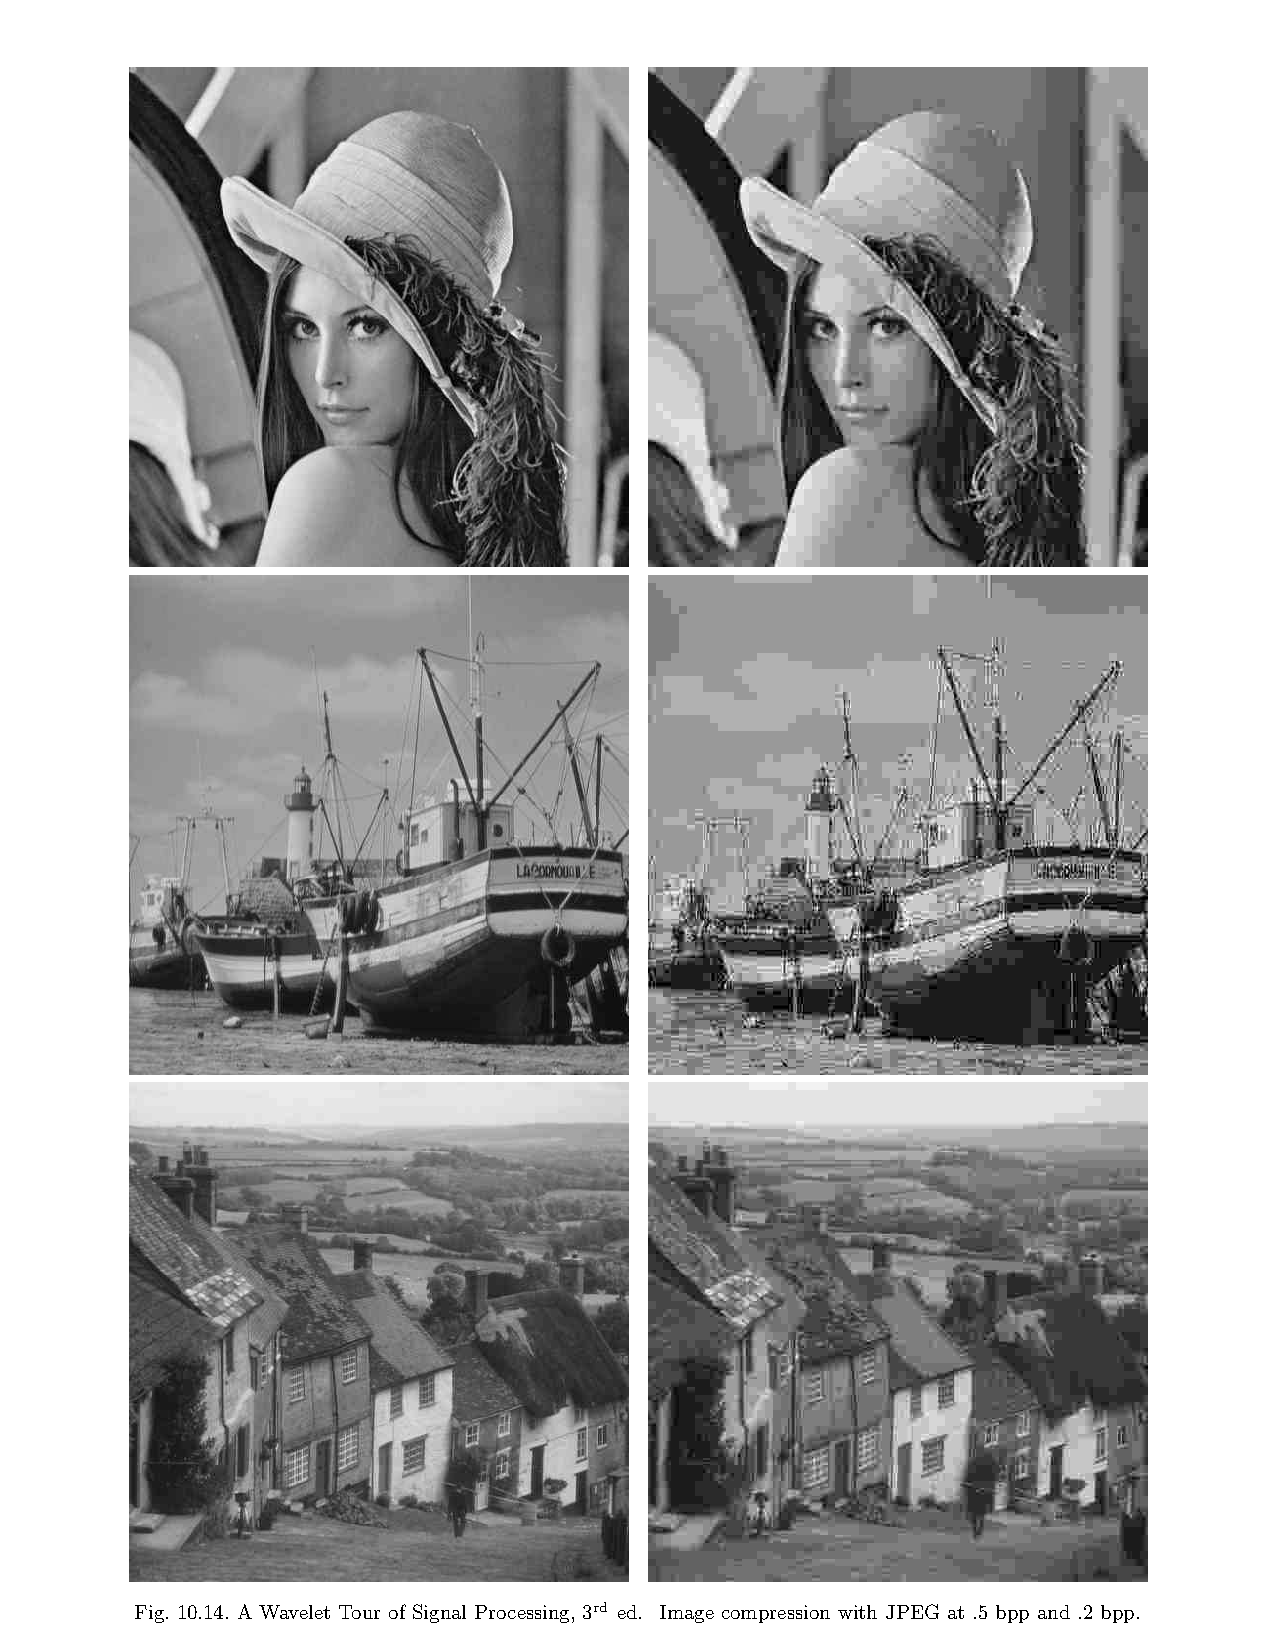
\includegraphics[width=\textwidth]{Figures/JPEG1}
\end{figure}
\newpage
\begin{figure}
\label{JPEG-12}
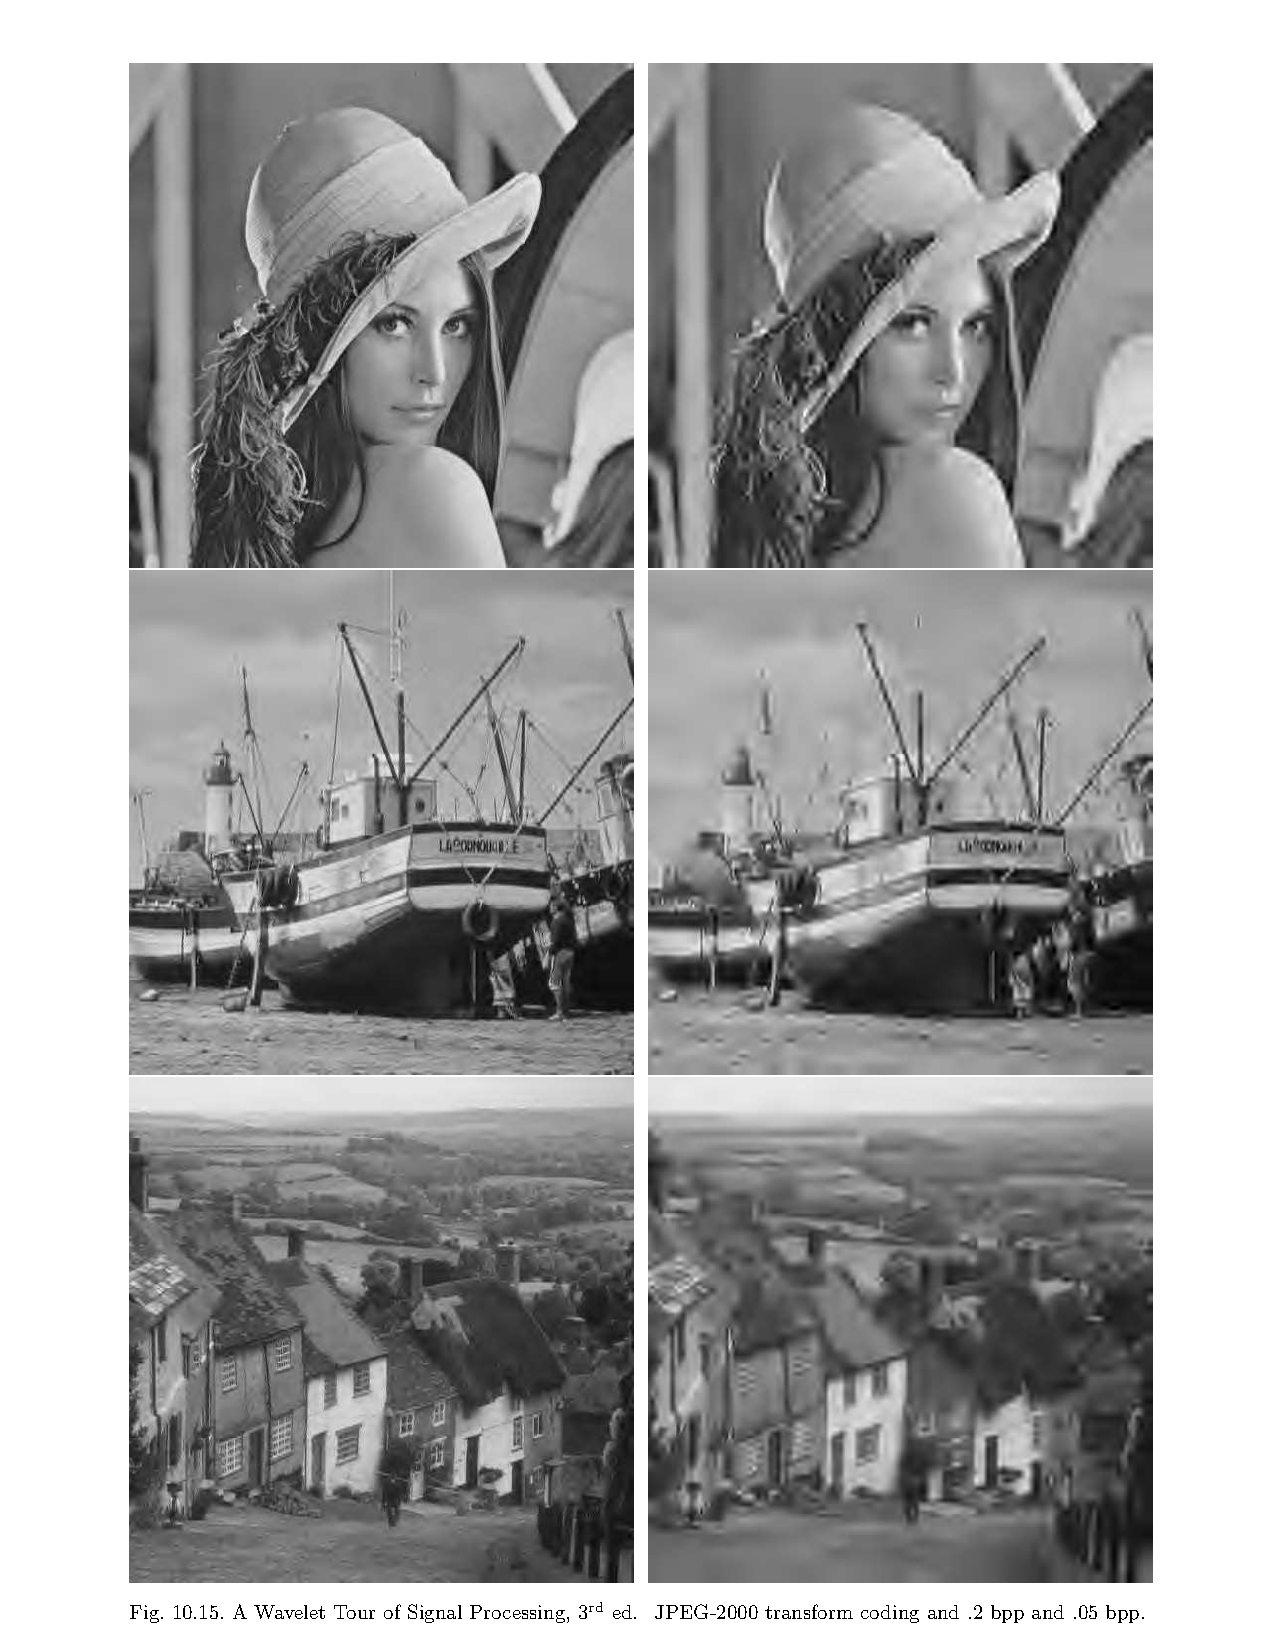
\includegraphics[width=\textwidth]{Figures/JPEG2}
\end{figure}





